%
% File naaclhlt2018.tex
%
%% Based on the style files for NAACL-HLT 2018, which were
%% Based on the style files for ACL-2015, with some improvements
%%  taken from the NAACL-2016 style
%% Based on the style files for ACL-2014, which were, in turn,
%% based on ACL-2013, ACL-2012, ACL-2011, ACL-2010, ACL-IJCNLP-2009,
%% EACL-2009, IJCNLP-2008...
%% Based on the style files for EACL 2006 by 
%%e.agirre@ehu.es or Sergi.Balari@uab.es
%% and that of ACL 08 by Joakim Nivre and Noah Smith

\documentclass[11pt,a4paper]{article}
\usepackage[hyperref]{naaclhlt2018}
\usepackage{times}
\usepackage{latexsym}

\usepackage{url}
\usepackage{graphicx} %package to manage images
\graphicspath{ {/} }

\aclfinalcopy % Uncomment this line for the final submission
%\def\aclpaperid{***} %  Enter the acl Paper ID here

\setlength\titlebox{6cm}
% You can expand the titlebox if you need extra space
% to show all the authors. Please do not make the titlebox
% smaller than 5cm (the original size); we will check this
% in the camera-ready version and ask you to change it back.

\newcommand\BibTeX{B{\sc ib}\TeX}

\title{A Scalable Augmentation of the Education Process}

\author{Bhairav Mehta \\
  University of Michigan \\
  {\tt bhairavm@umich.edu}
  \And
  Adithya Ramanathan \\
  University of Michigan \\
  {\tt adithram@umich.edu}}
\date{}

\begin{document}
\maketitle
\begin{abstract}
  Despite enormous progress in applications of machine learning and artificial intelligence, one of the slowest-adapting fields has been education. While collectively, we have expanded the accessibility to education through mediums such as MOOCs, these classrooms, albeit online, are still structured in the same format: lectures, written assignments, and grades. This paper starts from well-established hypotheses about effective student learning within the educational psychology community, and focuses in on the educational benefits of knowledge vocalizalization \cite{TODO}, parallel learning \cite{TODO}, and immediate feedback \cite{TODO}. We describe a novel intelligent tutoring system, which replicates many of the benefits cited in these hypotheses and provides a pipeline that allows our method to scale easily in terms of both class size and number of subjects, while still operating at the granularity of the needs of an individual. By harnessing free, online resources, combined with modern information retrieval and machine learning techniques, our system can be personalized towards any classroom. We provide full transparency to administrators and teachers, and allow them to provide the input and completely control or edit  decision made by the machine learning algorithms. Our initial experiments and pilot programs show promising results, and cement our hypothesis that our system is flexible enough to serve across a wide spectrum of purposes in a classroom setting.
\end{abstract}

\section{Introduction}

Education has always been a sequential process. Students learn algebra, geometry, and then calculus, and for some subjects, sequential learning offers a easy way to lay a natural foundation for future topics of study. Yet, in many cases, parallel learning of auxiliary yet related topics can help a student get through tough concepts \cite{TODO}. By providing a wider view of the topic in question, students gain more context, and can overcome mental roadblocks by bypassing them through temporarily focusing on other topics. Studying parallel areas can increase knowledge retention in the main focus, which has shown to be effective in not only humans \cite{TODO}, but has also inspired similar research geared towards artificial agents \cite{TODO}.

Even with parallel learning, the efficacy of learning depends highly on the study methods employed. Research on studying methods \cite{TODO} show that while highest in popularity, rote memorization and flashcards are among the worst performing in terms of knowledge retention. Methods that engage multiple sensory pipelines, such as those that require or return visual or audial information, are among the best performing. In particular, getting students to speak about what they know, and what they don't, can be shown to improve performance over long periods of time \cite{TODO}, especially when paired with getting feedback on what the student is saying. While rapid advances have been made in artificial speech systems \cite{TODO: Both Transcribing and Understanding}, rarely has this type of technology been applied to education.

Student learning is not a one-way street; in a ideal setting, when a student interacts with a learning system, she should also recieve feedback on the interaction. Education studies show that immediate feedback can help increase knowledge retention \cite{samuels_wu}. When compared to traditional delayed feedback methods such as grades on tests and quizzes, immediate feedback has been shown to improve understanding and comprehension. Both parallel learning and immediate feedback in education have empirically shown to increase the value of time spent in the classroom, but are idealistic by nature. Traditionally, education is more efficient as a one-size-fits-all system, but as a result doesn't scale to operate at the granularity of individual students. 

We can see this embodiment of parallel learning, vocalization, and immediate feedback, as well as their benefits, in student tutors. Tutors in primary schools and universities are often top students in their classes to begin with \cite{TODO}, but can later on outperform their peers from the same performance group \cite{TODO}. Our hypothesis is that by coming up with alternative methods to explain tough concepts to other students (i.e through analogies or related material), as well as constantly talking about the topic and getting feedback from their students, allows them to better solidify their own understanding of the concepts, and therefore drives them to true mastery rather than just good grades. 

We develop the framework that takes initial steps in providing a solution to these issues that hinder the efficiency of our educational institutions. We present a system that extracts the key concepts from bodies of expert-curated raw text and internet sources, and use these key phrases as a proxy for the knowledge a student hopes to gain from the particular group of sources. When presented with an answer, the system presents the student with feedback, our system uses an internal similarity metric to deduce what concepts the student is struggling with, and offers recommendations of other topics within that class to study in parallel in order to improve knowledge retention of the main task. We stay true to the unofficial education-technology motto of minimizing teacher investment while maximizing student impact, and we conclude by offering future ideas on implementations and improvements of this system.

\section{Related Work}
% Intelligent Tutoring Systems = 1 paragraph
% NER / RE / NLU = 2 sentences

Natural Language Understanding, a subset of Natural Language Processing, involves training computers to understand unstructured text. While considered an AI-Hard problem, a more accessible subset of this area is concerned with Information Extraction, or the task of retrieving structured information from unstructured data sources, such as raw text, images, or even video. Structured information, especially in a text-based setting, is often represented in the form entities and relationships. 

Named Entity Recognition (NER) is a subset of information extraction and involves locating and classifying named entities in text into pre-defined categories such as the names of persons, organizations, locations, etc. Today’s NER systems achieve near-human performance on popular datasets \cite{M98-1002}, but are often brittle and susceptible to the domain-transfer problem \cite{Poibeau01propername}. This puts an onus on the researcher to provide the model with a labelled, relevant dataset, and currently, even with the state-of-the-art models \cite{Turian:2010:WRS:1858681.1858721} \cite{Lin:2009:PCD:1690219.1690290}, the domain transfer issue remains unsolved. In our work, we deal with examples for which we have labelled datasets that are related to the target domain.

%  Can we use this to score??
Relationship Extraction (RE) involves understanding how two entities are related. For example, a sentence “John works at XYZ” may translate into “PERSON works for ORGANIZATION”, with “works for” being the relation. Relationships are important in learning how much entities semantically mean to each other, and can stronger relationships can serve as a proxy for more importance of one entity to the other. Specifically, relationship extraction from raw text can be used to build knowledge graphs \cite{Ramakrishnan:2006:FSR:2127045.2127088}. Knowledge graphs often hold facts as relationships, and in question-answering systems, can quickly infer answers by traversing relevant relationships between the entities in question. Knowledge graphs are important parts of other products like personal assistants, but to our knowledge, have not been directly applied to helping people in the traditional education process.

Education technology (ET) is defined as the "the study and ethical practice of facilitating learning and improving performance by creating, using, and managing appropriate technological processes and resources" \cite{hlynka_jacobsen}. Main issues cited by educators of unsuccessful education technology have centered around transparency, startup cost, and narrowness of scope \cite{TODO}: Educators felt completely pushed aside, were asked to spend unreasonable amounts of time with setup, or were given a specific application with limited scope; all of which are detrimental to user adoption. Education technology takes many forms, and while diverse in implementation, many educators agree that the ideal software solution will involve minimal teacher effort while still providing a substantial impact to students \cite{norris_soloway02/12/18}. Some of the best ET applications on the market, including Duolingo and \cite{!!!textbook websiteTODO}, do just this: they offer flexibility in both their scope and curiculum and allow the educator to determine their importance in the classroom. They constantly interact with the student in multiple ways, and offer ease of setup through prebuilt curicula. Yet, while leaders in ET, they are still constrained by the fact that their courses are entirely expert-curated. Our approach builds on the common characteristics shared by these applications by augmenting and automating menial parts of the process, all while keeping the "teacher-in-the-loop" mentality.

\section{Methodology}
The system is constructed using five key steps. In order, the steps are as following: Raw Text Extraction, Named Entity Recognition, Topic Scoring / Ranking, Questioning / Answering, and Knowledge Graph Querying.

\subsection{Datasets}
% Turn Datasets + Raw Text + GMB = 2 sentences
Data was pulled and annotated from two main sources. Raw text was acquired by scraping Wikipedia using a seedlist of topics. Additionally, data used to train the Named Entity Recognition model was pulled using an annotated version of Groningen Meaning Bank. 

\subsubsection{Raw Text}\label{data_raw_text}
Raw text is extracted by providing a seed list of URLs to a traditional, web-crawling spider, and the HTML on each page is processed and the raw text is extracted using the \texttt{BeautifulSoup} library. Our spider performs a depth-2 search from the seed URLs, meaning that it adds the links on the pages with the seed URLs, and then performs that process recursively on the next level as well. The assumption that we make is that a human expert provides these seed URLs by judging that the seed URLs are in fact relevant to the questions that will be inputted into the system at a later time.

\subsubsection{Annotated Groningen Meaning Bank}
The Groningen Meaning Bank(GMB) was developed at the University of Groningen \cite{Bos2017GMB}. The bank itself features thousands of texts which have been tokenized, tagged for parts of speech and tagged for lexical categories. The specific dataset used in this project is a further annotated version of the typical GMB and features labels for each term in the text in the form of named entity labels. Specifically, for this use case, terms are labelled using one of the following labels: geo (Geographical Entity), org (Organization), per (Person), gpe (Geopolitical Entity), tim (Time Indicator), art (Artifact), eve (Event), nat (Natural Phenomenon), O (Other). The dataset was tremendously useful as it provided a direct parallel to the output we wished to generate via our model. However, enhancements to the dataset do persist. Specifically, one area in which we may have benefitted from variation within the dataset is in the form of grouping of multi-term named entities. Currently, the system predicts upon raw text using data examples pulled from this bank, and each individual term is associated with named entity tag. This however, fails to consider that certain named entities are constructed of multiple terms. For example, the term ‘Second Continental Congress’ is considered to be three unique named entities by this corpus rather than one large, multi term named entity. 

\subsection{System}
\subsubsection{Raw Text Extraction}
Using the raw text harvested from the spider described in Section \ref{data_raw_text}, we remove stopwords, and stem the remaining text using the NLTK Wordnet Lemmatizer \cite{Fellbaum1998}. With this preprocessed text, we concatenate all of the web pages to generate a tf-idf index \cite{Ramos_usingtf-idf}. As we assume that our text samples are representative of the true distribution of words, our tf-idf index serves as a proxy of how important and rare particular words are to the whole of the corpus. Through experimentation testing the ability of these indices to transfer across domains (i.e having been generated on a list of seed URLs from American History, how accurately could we gauge the importance of words from Psychology text), we find that these indices are also subject to the domain transfer issue discussed in the Related Work. To mitigate this issue, we envision a tf-idf index being generated per subject (i.e History, Psychology, etc).

\subsubsection{Named Entity Recognition}
The Named Entity module is utilized in two phases. First, there is a training phase where the model is trained to predict named entities in raw text using the Annotated Groningen Meaning Base as a training corpus. Secondly, there is a classification phase where the trained model is stored into a pickle file, and utilized to predict named entities from raw text. 

Training begins with preprocessing and feature engineering of the training corpus. The corpus is preprocessed into sentence tuples. The entire training corpus is reconstructed as a list of tuples, where each sentence is broken down into tuples of word, part-of-speech, and it’s respective named entity tag. Given this reformatted training corpus, the data is converted into features extracting certain key identifiers for each word in a sentence such as case, position, part-of-speech, contextual part-of-speech, whether the word is a number, and whether the word is a title. Additionally, the features are engineered to consider both the previous and next word, and their respective values as features as well.  At this point, the system has reformatted the Annotated Groningen Meaning Base into a collection of feature vectors. 

For our use case, we utilize a Conditional Random Fields model. The CRF model performs a class of statistical modeling focused on conditional probability modeling. Additionally, CRF models fall into the class of sequential models, and is thus effective in this use case by considering neighboring terms and context when making conditional probability based predictions. The model is trained using the feature vectors previously constructed. The feature map appears as follows:

$$\phi(x_1, ...,x_m, s_1,...,s_m)$$ where $x \in$ feature vectors and $s \in $ named entity labels.

The feature vectors are processed and considered using a log likelihood function:
$$L(w) = \sum_{i=1}^{n}log(p(s^i|x^i; w) - \frac{\lambda_2}{2} ||w||^2_2 - \lambda_1||w||_1$$

Where the conditional probability function is modeled as:
$$p(s|x;w) = \frac{exp(w \cdot \phi(x,s))}{\sum_{s'}exp(w \cdot \phi(x,s'))}$$

And the parameter vector, where the two parameter terms (which helps alleviate complexity) are:
$$\frac{\lambda_2}{2} ||w||^2_2$$ $$\lambda_1||w||_1$$

The parameter vector is estimated as:
$$w^* = \arg\max_{w\in \mathbb{R}^d}L(w)$$

Based on training, and cross validation tests, we chose to modify the L1 Hyperparameter by increasing the value. This helped the model further focus on context rather than pure memorization and led to better empirical results. Once the model has been trained, we dump the model into a pickle file. The pickle file serves as a saved, binary export of the model such that we can later access the model to make predictions rather than retraining the model at each occurrence. 

The second phase begins by taking in raw text as input. This raw text is then split into sentences, and each sentence is then further broken down into tuples. Using the NLTK (Natural Language Toolkit) library, the part-of-speech tagger is utilized to breakdown the sentence into tuples of term, and part of speech. At this point, we convert these reformatted sentences into feature vectors, in the exact same manner as the training data. We then make predictions regarding each term.If the parameter vector is estimated, the most likely tag for a label can be found using.
$$s^* = argmax_{s}p(s|x;w^*)$$

At this point, we parse out all terms that are not considered named entities, and soley keep those original terms that are considered to be named entities. 
\subsubsection{Topic Scoring and Ranking}

Now, given a trained NER system and a tf-idf index that will serve as a proxy for importance, we can start to evaluate our system. During deployment, we envision that this is the first step an actual teacher would be involved. 

The system prompts the user for a question title (which will be shown to the student), and then asks the user to provide source documents that the expert user deems to be relevant to the question posed. The source documents can be raw text, or URLs which are preprocessed the same way as described in Section  \ref{data_raw_text}. From there, we run each processed word through a scoring module

$$score_q(w) = tfidf(w) + a*SI(w) + b*NE(w)$$

where $SI(w)$, short for semantic importance, is a multiplier if the particular word was in a section heading in the original HTML and a constant if from raw text, $NE(w)$ is a multiplier if the word is present in any of the named entities extracted from the text using the NER model, and $a$ and $b$ are empirically defined hyperparameters. If the word comes from raw text inputted by the user, $SI(w)>1$, using the assumption that the user would have only inserted that text excerpt if it was actually relevant, whereas websites can contain lots of incorrect information. In addition, if the word is found inside of a named entity, we replace the word with the named entity itself. We then associate a thresholded list of \texttt{\{word: score\}} pairs to the question, which serve as the “key concepts” associated with the question. 

\subsubsection{Teacher-in-the-Loop}
In a deployed version of the system, we envision the sorted \texttt{\{word: score\}} pairs to be returned to the user, and tweaked as necessary using expert knowledge.


\subsubsection{Question and Answer System}
At this point, the system would be turned to the user, and the question inputted by the teacher would be posed to the student. In this preliminary work, we take a naive approach to the student scoring problem, awarding points to the student by the following criteria:

\begin{center}
    \begin{align}
        score_s(A) =\\
        \sum_{w_i \in A} \sum_{w_j \in E}[[w_i==w_j]]* score_q(w_j)
	\end{align}
\end{center}

where $A$ is a tokenized version of the students answer, and $E$ is a tokenized version of the named entities generated from the teacher inputs the question.

This scoring methodology forces students to have exact answers, which is not ideal for educational software. While simple, future work could explore the use of synonyms, and words that have related meaning to those that come in as the student response for the use of scoring.

\subsubsection{Knowledge Graph Querying} 
% TODO: Turn into a similarity metric of scores + word pairs, and how to rank them; Remove API
The knowledge graph is utilized in the project in an effort to take advantage of the concept of adjacent learning. As such, we utilize the constructed Google Knowledge Graph, and its corresponding API to access adjacent topics. Given that a student misses a certain concept when participating with the question answer system, these missed concepts are utilized as the terms with which we query the Google Knowledge Graph. We threshold the responses from the API request to the five most adjacent responses. These responses are then returned to the user as other suggested topics that would help the user better understand the material. Future implementations would utilize more specific corpuses to construct subject-specific knowledge graphs, for more relevant results to the user.

\subsubsection{Voice}
% TODO 


\subsection{Use Cases}
% Also talk about range of spectrum -- gives the teacher back time!
The use case we envision for our project is a student begins interaction with the system. At this point, the system asks the user a question such as “Tell me about how World War II began?”. The student then responds to this query by dictating all of the different pieces of information that they believe is relevant to answering this question. The system compares this information provided by the user against an internal scored, ranked list of terms relevant to the answer to the original question. Any terms that are ranked by the system, but missed by the student are then returned to the user as topics worth studying further. Additionally, the missed topics are input into a  knowledge graph query such that topics related to the missed piece of information are also provided to the student.

In this way, our system targets specific weaknesses within a students domain knowledge of a subject. The system itself can be constructed for specific classroom curriculums, and provides an extension of the teacher to the student that allows the student to study more effectively when outside of the classroom itself.  

\section{Experiments}
%  Need NER Validation, User Study for Extracted Topics Relevance, User Study for Related Topics,
%  TODO: Add in something about US History (and why)
To evaluate results we performed 5-Folds Cross Validation to understand performance of our conditional random field model, utilized for named entity prediction. Additionally, to evaluate the system as a whole, which heavily depends on relevance feedback and a question answering system, we constructed an experiment in the form of a user study to understand the effectiveness of the system in serving as a study aid to students. 

The 5 folds cross validation involves multiple rounds of random partitioning. Each round of partitioning involves separation into one training partition and one validation partition. The model is constructed using the training partition and tested using the validation partition. This process is repeated for each round and the results are averaged together. The randomness of the construction by design helps alleviate worries in the form of overfitting or underfitting. The model itself performed relatively well in cross validation testing. Certain key takeaways are still found however. Primarily, the data appears to be significantly dependent on the number of samples for each named entity type. Additionally, the system struggles with recall while performing relatively well in terms of precision.

\begin{figure}[h!]
    \centering
    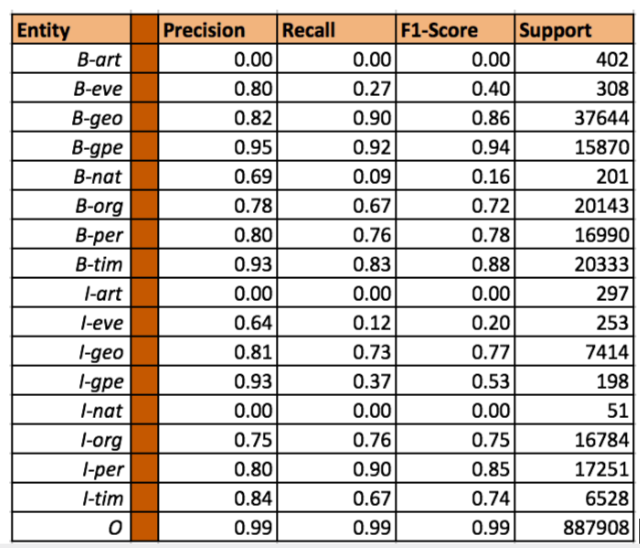
\includegraphics[h!,width=0.4\textwidth]{5folds.png}
    \caption{5-Folds Cross Validation of NER}
    \label{fig:5folds}
\end{figure}

The user study was constructed to evaluate system performance on 5 example questions, and judged by 12 respondents. Each batch of 4 respondents was additionally averaged for an average evaluation score for the system. The user study resulted in a great variety of results, and has lead us to consider many further system enhancements in an effort to alleviate some of the concerns pointed out by this user study.

\begin{table}[h!]
\centering
\begin{tabular}{c}
\hline \bf Questions Asked \\ \hline
Who was George Washington? \\
Name some important events in the Rev. War \\
How was life for the Iriquois Indians?\\
How did World War II Start? \\
What were some reasons for the Civil War? \\
\hline
\end{tabular}
\caption{\label{ques-table} Questions Asked During User Study}
\end{table}

In the user study, whose results can be seen in Appendix A, it can be seen that the system performs well when dealing with questions 4 and 5. However, when considering the ratings related to questions 1 and 3, the system has drastically worse performance. The results themselves are empirically obvious of the shortcomings. When looking at the related, suggested topics (as returned by the knowledge graph), a query for ‘George Washington’ returns results related to completely unrelated topics to the question such as ‘George Washington University’. This completely unrelated response is representative of a key problem with the system - the knowledge graph has no specific contextual awareness. One potential solution to this problem would be an additional layer of post processing added to the knowledge graph module. Rather than relaying the first 5 responses from the knowledge query, the system should perhaps be capable of considering the returned responses and only relating those responses considered to actually be relevant. 

\section{Conclusion and Future Work}

We present an alternative education solution through the use of modern information retrieval and machine learning techniques as described above. Our system can scale easily to many classes and to unlimited numbers of students By harnessing the depth and breadth of resources available online, in combination with methodology that helps establish adjacent learning with immediate feedback, proven solutions to educational problems are being implemented. While the system as it stands provides the foundation for a framework focused on this education pipeline, glaring possibilities for improvement still exist. For example, related topics as returned by our internal similarity metric are not always intuitive or useful. Future work could also explore

\bibliography{naaclhlt2018}
\bibliographystyle{acl_natbib}

\appendix

\section{Appendix: Results from User Study}

In Table \ref{user-table}, we see the relevance ranking of the topics returned by the knowledge graph, when supplied the questions from Table \ref{ques-table}. We then ask our users to rank the relevance of the top five returned topics, with 1 being the worst and 5 being the best. Some topics work better than others, due to the wide array of knowledge that Google's knowledge graph contains when compared to our controlled experiments. We believe that future work can help mitigate some of the low ranking responses by recommending relevant \textit{questions} from the class that the current question is also in, rather than querying an outside API.

\begin{table}[h!]
\begin{tabular}{|c|c|c|c|c|c|}
    \hline \bf User & \bf Q1 & \bf Q2 & \bf Q3 & \bf Q4 & \bf Q5 \\  
    \hline
    \bf 1 & 1 & 3 & 2 & 4 & 4 \\ 
    \bf 2 & 2 & 3 & 2 & 5 & 4 \\ 
    \bf 3 & 1 & 4 & 2 & 3 & 3 \\ 
    \bf 4 & 1 & 3 & 2 & 4 & 4 \\ 
    \bf 5 & 2 & 5 & 2 & 5 & 4 \\ 
    \bf 6 & 1 & 3 & 2 & 5 & 5 \\ 
    \bf 7 & 2 & 3 & 1 & 4 & 4 \\ 
    \bf 8 & 1 & 3 & 2 & 4 & 4 \\ 
    \bf 9 & 1 & 4 & 3 & 5 & 4 \\ 
    \bf 10 & 1 & 3 & 2 & 4 & 3 \\ 
    \bf 11 & 2 & 3 & 2 & 5 & 4 \\ 
    \bf 12 & 1 & 4 & 2 & 5 & 4 \\ 
    \hline
    \bf Average & \bf 1.33 & \bf 3.42 & \bf 2.00 & \bf 4.42 & \bf 3.92 \\ 
    \hline
\end{tabular}
\caption{\label{user-table} Questions Asked During User Study}
\end{table}
\end{document}